\documentclass[twoside]{book}

% Packages required by doxygen
\usepackage{fixltx2e}
\usepackage{calc}
\usepackage{doxygen}
\usepackage[export]{adjustbox} % also loads graphicx
\usepackage{graphicx}
\usepackage[utf8]{inputenc}
\usepackage{makeidx}
\usepackage{multicol}
\usepackage{multirow}
\PassOptionsToPackage{warn}{textcomp}
\usepackage{textcomp}
\usepackage[nointegrals]{wasysym}
\usepackage[table]{xcolor}

% Font selection
\usepackage[T1]{fontenc}
\usepackage[scaled=.90]{helvet}
\usepackage{courier}
\usepackage{amssymb}
\usepackage{sectsty}
\renewcommand{\familydefault}{\sfdefault}
\allsectionsfont{%
  \fontseries{bc}\selectfont%
  \color{darkgray}%
}
\renewcommand{\DoxyLabelFont}{%
  \fontseries{bc}\selectfont%
  \color{darkgray}%
}
\newcommand{\+}{\discretionary{\mbox{\scriptsize$\hookleftarrow$}}{}{}}

% Page & text layout
\usepackage{geometry}
\geometry{%
  a4paper,%
  top=2.5cm,%
  bottom=2.5cm,%
  left=2.5cm,%
  right=2.5cm%
}
\tolerance=750
\hfuzz=15pt
\hbadness=750
\setlength{\emergencystretch}{15pt}
\setlength{\parindent}{0cm}
\setlength{\parskip}{3ex plus 2ex minus 2ex}
\makeatletter
\renewcommand{\paragraph}{%
  \@startsection{paragraph}{4}{0ex}{-1.0ex}{1.0ex}{%
    \normalfont\normalsize\bfseries\SS@parafont%
  }%
}
\renewcommand{\subparagraph}{%
  \@startsection{subparagraph}{5}{0ex}{-1.0ex}{1.0ex}{%
    \normalfont\normalsize\bfseries\SS@subparafont%
  }%
}
\makeatother

% Headers & footers
\usepackage{fancyhdr}
\pagestyle{fancyplain}
\fancyhead[LE]{\fancyplain{}{\bfseries\thepage}}
\fancyhead[CE]{\fancyplain{}{}}
\fancyhead[RE]{\fancyplain{}{\bfseries\leftmark}}
\fancyhead[LO]{\fancyplain{}{\bfseries\rightmark}}
\fancyhead[CO]{\fancyplain{}{}}
\fancyhead[RO]{\fancyplain{}{\bfseries\thepage}}
\fancyfoot[LE]{\fancyplain{}{}}
\fancyfoot[CE]{\fancyplain{}{}}
\fancyfoot[RE]{\fancyplain{}{\bfseries\scriptsize Generated by Doxygen }}
\fancyfoot[LO]{\fancyplain{}{\bfseries\scriptsize Generated by Doxygen }}
\fancyfoot[CO]{\fancyplain{}{}}
\fancyfoot[RO]{\fancyplain{}{}}
\renewcommand{\footrulewidth}{0.4pt}
\renewcommand{\chaptermark}[1]{%
  \markboth{#1}{}%
}
\renewcommand{\sectionmark}[1]{%
  \markright{\thesection\ #1}%
}

% Indices & bibliography
\usepackage{natbib}
\usepackage[titles]{tocloft}
\setcounter{tocdepth}{3}
\setcounter{secnumdepth}{5}
\makeindex

% Hyperlinks (required, but should be loaded last)
\usepackage{ifpdf}
\ifpdf
  \usepackage[pdftex,pagebackref=true]{hyperref}
\else
  \usepackage[ps2pdf,pagebackref=true]{hyperref}
\fi
\hypersetup{%
  colorlinks=true,%
  linkcolor=blue,%
  citecolor=blue,%
  unicode%
}

% Custom commands
\newcommand{\clearemptydoublepage}{%
  \newpage{\pagestyle{empty}\cleardoublepage}%
}

\usepackage{caption}
\captionsetup{labelsep=space,justification=centering,font={bf},singlelinecheck=off,skip=4pt,position=top}

%===== C O N T E N T S =====

\begin{document}

% Titlepage & ToC
\hypersetup{pageanchor=false,
             bookmarksnumbered=true,
             pdfencoding=unicode
            }
\pagenumbering{roman}
\begin{titlepage}
\vspace*{7cm}
\begin{center}%
{\Large get geo }\\
\vspace*{1cm}
{\large Generated by Doxygen 1.8.11}\\
\end{center}
\end{titlepage}
\clearemptydoublepage
\tableofcontents
\clearemptydoublepage
\pagenumbering{arabic}
\hypersetup{pageanchor=true}

%--- Begin generated contents ---
\chapter{Namespace Index}
\section{Packages}
Here are the packages with brief descriptions (if available)\+:\begin{DoxyCompactList}
\item\contentsline{section}{\hyperlink{namespace_contour___e_t}{Contour\+\_\+\+E\+T} }{\pageref{namespace_contour___e_t}}{}
\item\contentsline{section}{\hyperlink{namespacedocutil__text}{docutil\+\_\+text} }{\pageref{namespacedocutil__text}}{}
\item\contentsline{section}{\hyperlink{namespace_d_r___e_c}{D\+R\+\_\+\+E\+C} }{\pageref{namespace_d_r___e_c}}{}
\item\contentsline{section}{\hyperlink{namespaceet__util}{et\+\_\+util} }{\pageref{namespaceet__util}}{}
\item\contentsline{section}{\hyperlink{namespace_flag_analysis}{Flag\+Analysis} }{\pageref{namespace_flag_analysis}}{}
\item\contentsline{section}{\hyperlink{namespacegap_tests}{gap\+Tests} }{\pageref{namespacegap_tests}}{}
\item\contentsline{section}{\hyperlink{namespaceheatmap__slopes}{heatmap\+\_\+slopes} }{\pageref{namespaceheatmap__slopes}}{}
\item\contentsline{section}{\hyperlink{namespaceheatmap__subplots}{heatmap\+\_\+subplots} }{\pageref{namespaceheatmap__subplots}}{}
\item\contentsline{section}{\hyperlink{namespaceoptimum__growing__season}{optimum\+\_\+growing\+\_\+season} }{\pageref{namespaceoptimum__growing__season}}{}
\item\contentsline{section}{\hyperlink{namespace_preprocess}{Preprocess} \\*E\+T }{\pageref{namespace_preprocess}}{}
\item\contentsline{section}{\hyperlink{namespace_preprocess_01_d_r}{Preprocess D\+R} }{\pageref{namespace_preprocess_01_d_r}}{}
\item\contentsline{section}{\hyperlink{namespace_preprocess_01_e_t}{Preprocess E\+T} }{\pageref{namespace_preprocess_01_e_t}}{}
\item\contentsline{section}{\hyperlink{namespaces__post__process}{s\+\_\+post\+\_\+process} }{\pageref{namespaces__post__process}}{}
\end{DoxyCompactList}

\chapter{Hierarchical Index}
\section{Class Hierarchy}
This inheritance list is sorted roughly, but not completely, alphabetically\+:\begin{DoxyCompactList}
\item \contentsline{section}{Frame}{\pageref{class_frame}}{}
\begin{DoxyCompactList}
\item \contentsline{section}{get\+\_\+geo\+\_\+\+H\+U\+C.\+Application}{\pageref{classget__geo___h_u_c_1_1_application}}{}
\end{DoxyCompactList}
\item \contentsline{section}{get\+\_\+geo\+\_\+\+H\+U\+C.\+geo}{\pageref{classget__geo___h_u_c_1_1geo}}{}
\end{DoxyCompactList}

\chapter{Class Index}
\section{Class List}
Here are the classes, structs, unions and interfaces with brief descriptions\+:\begin{DoxyCompactList}
\item\contentsline{section}{\hyperlink{classget__geo___h_u_c_1_1_application}{get\+\_\+geo\+\_\+\+H\+U\+C.\+Application} }{\pageref{classget__geo___h_u_c_1_1_application}}{}
\item\contentsline{section}{\hyperlink{class_frame}{Frame} }{\pageref{class_frame}}{}
\item\contentsline{section}{\hyperlink{classget__geo___h_u_c_1_1geo}{get\+\_\+geo\+\_\+\+H\+U\+C.\+geo} }{\pageref{classget__geo___h_u_c_1_1geo}}{}
\end{DoxyCompactList}

\chapter{File Index}
\section{File List}
Here is a list of all files with brief descriptions\+:\begin{DoxyCompactList}
\item\contentsline{section}{\hyperlink{_contour___e_t_8py}{Contour\+\_\+\+E\+T.\+py} }{\pageref{_contour___e_t_8py}}{}
\item\contentsline{section}{\hyperlink{docutil__text_8py}{docutil\+\_\+text.\+py} }{\pageref{docutil__text_8py}}{}
\item\contentsline{section}{\hyperlink{_d_r___e_c_8py}{D\+R\+\_\+\+E\+C.\+py} }{\pageref{_d_r___e_c_8py}}{}
\item\contentsline{section}{\hyperlink{et__util_8py}{et\+\_\+util.\+py} }{\pageref{et__util_8py}}{}
\item\contentsline{section}{\hyperlink{_flag_analysis_8py}{Flag\+Analysis.\+py} }{\pageref{_flag_analysis_8py}}{}
\item\contentsline{section}{\hyperlink{gap_tests_8py}{gap\+Tests.\+py} }{\pageref{gap_tests_8py}}{}
\item\contentsline{section}{\hyperlink{heatmap__slopes_8py}{heatmap\+\_\+slopes.\+py} }{\pageref{heatmap__slopes_8py}}{}
\item\contentsline{section}{\hyperlink{heatmap__subplots_8py}{heatmap\+\_\+subplots.\+py} }{\pageref{heatmap__subplots_8py}}{}
\item\contentsline{section}{\hyperlink{optimum__growing__season_8py}{optimum\+\_\+growing\+\_\+season.\+py} }{\pageref{optimum__growing__season_8py}}{}
\item\contentsline{section}{\hyperlink{_preprocess_01_d_r_8py}{Preprocess D\+R.\+py} }{\pageref{_preprocess_01_d_r_8py}}{}
\item\contentsline{section}{\hyperlink{_preprocess_01_e_t_8py}{Preprocess E\+T.\+py} }{\pageref{_preprocess_01_e_t_8py}}{}
\item\contentsline{section}{\hyperlink{s__post__process_8py}{s\+\_\+post\+\_\+process.\+py} }{\pageref{s__post__process_8py}}{}
\end{DoxyCompactList}

\chapter{Namespace Documentation}
\hypertarget{namespaceget__geo___h_u_c}{}\section{get\+\_\+geo\+\_\+\+H\+UC Namespace Reference}
\label{namespaceget__geo___h_u_c}\index{get\+\_\+geo\+\_\+\+H\+UC@{get\+\_\+geo\+\_\+\+H\+UC}}
\subsection*{Classes}
\begin{DoxyCompactItemize}
\item 
class \hyperlink{classget__geo___h_u_c_1_1_application}{Application}
\item 
class \hyperlink{classget__geo___h_u_c_1_1geo}{geo}
\end{DoxyCompactItemize}
\subsection*{Functions}
\begin{DoxyCompactItemize}
\item 
def \hyperlink{namespaceget__geo___h_u_c_a00508deb9e21d5ff5be209dada8cb9fd}{create\+Widgets} (\hyperlink{namespaceget__geo___h_u_c_a5d34137420af63fc8dd32374dead14a8}{self})
\item 
def \hyperlink{namespaceget__geo___h_u_c_a400d7645bf5f9b8f5a07cd60f749d1b7}{get\+\_\+geo} (\hyperlink{namespaceget__geo___h_u_c_a5d34137420af63fc8dd32374dead14a8}{self}, args)
\item 
def \hyperlink{namespaceget__geo___h_u_c_a4d0dce07eab2a159ef5d04e0742d5e03}{is\+\_\+number} (\hyperlink{namespaceget__geo___h_u_c_a5d34137420af63fc8dd32374dead14a8}{self}, s)
\item 
def \hyperlink{namespaceget__geo___h_u_c_a4464d7f0ff14cfe91f0b14a490327af9}{\+\_\+\+\_\+init\+\_\+\+\_\+} (\hyperlink{namespaceget__geo___h_u_c_a5d34137420af63fc8dd32374dead14a8}{self}, master=None)
\item 
def \hyperlink{namespaceget__geo___h_u_c_ab68d25f6902e2500c520513afb9253f2}{geocode} (\hyperlink{namespaceget__geo___h_u_c_a5d34137420af63fc8dd32374dead14a8}{self}, \hyperlink{namespaceget__geo___h_u_c_acafcc8295c3d6a0de2fb561809cca132}{latlng}, \hyperlink{namespaceget__geo___h_u_c_abd10e556b8081f3cd80bff1a987455af}{sensor}, geo\+\_\+args)
\item 
def \hyperlink{namespaceget__geo___h_u_c_ad7a7e36924d7182d2e06569e3abb5ea7}{huccode} (\hyperlink{namespaceget__geo___h_u_c_a5d34137420af63fc8dd32374dead14a8}{self}, \hyperlink{namespaceget__geo___h_u_c_ac22be281ee4954369c420f4045ec3336}{dms\+\_\+lat}, \hyperlink{namespaceget__geo___h_u_c_a3db416386a0a3ae6cf4b30fab0f65118}{dms\+\_\+lon}, huc\+\_\+args)
\item 
def \hyperlink{namespaceget__geo___h_u_c_ace8718ec9f6ab42ef73d183f38576100}{convert\+\_\+dms} (\hyperlink{namespaceget__geo___h_u_c_a5d34137420af63fc8dd32374dead14a8}{self}, d, m, s)
\item 
def \hyperlink{namespaceget__geo___h_u_c_a79b57d5406de0fef5ee616514de74584}{convert\+\_\+dec\+\_\+tude} (\hyperlink{namespaceget__geo___h_u_c_a5d34137420af63fc8dd32374dead14a8}{self}, decimal)
\item 
def \hyperlink{namespaceget__geo___h_u_c_a25d58c7f5b75b8d09a4738ec01a0e312}{convert\+\_\+dec\+\_\+lat\+\_\+lon} (\hyperlink{namespaceget__geo___h_u_c_a5d34137420af63fc8dd32374dead14a8}{self}, decimal, tude)
\end{DoxyCompactItemize}
\subsection*{Variables}
\begin{DoxyCompactItemize}
\item 
\hyperlink{namespaceget__geo___h_u_c_a7592d1dc926835f8c651c5761a3cf94a}{location}
\item 
\hyperlink{namespaceget__geo___h_u_c_ada77bf554a2fd51d028bc3830983b8b6}{text}
\item 
\hyperlink{namespaceget__geo___h_u_c_aa7eddbf5988aec86b6750fa36bf532be}{e}
\item 
\hyperlink{namespaceget__geo___h_u_c_a5d34137420af63fc8dd32374dead14a8}{self}
\item 
\hyperlink{namespaceget__geo___h_u_c_ad4f932dfe1b13e5124bc8be92dfb1f07}{width}
\item 
\hyperlink{namespaceget__geo___h_u_c_a6756d51ec2f6d391eddbc37c88a3369c}{b}
\item 
\hyperlink{namespaceget__geo___h_u_c_a8aad6d9263e79de308254e23bad82c50}{command}
\item 
\hyperlink{namespaceget__geo___h_u_c_a49b3d33e0540c2e2f9e991370aae8f8e}{cnty\+\_\+lab}
\item 
\hyperlink{namespaceget__geo___h_u_c_a3cbe3b2d0670a061bbc0c7be84c34d33}{result} = geo.\+simplejson.\+load(geo.\+urllib.\+urlopen(\hyperlink{namespaceget__geo___h_u_c_ab6098a8720c14d3cf3f34a3301c2ca93}{url}))
\item 
\hyperlink{namespaceget__geo___h_u_c_a5e43010bf41ec0eb1eb43403e310e26e}{t}
\item 
\hyperlink{namespaceget__geo___h_u_c_ac67b3377ef85a8077485ef5ae2c64c59}{textvariable}
\item 
\hyperlink{namespaceget__geo___h_u_c_adae93ea1e2d42a6d3c9992ae2e2277a0}{huc\+\_\+lab}
\item 
\hyperlink{namespaceget__geo___h_u_c_a68717ed78e37a7292f01cf4e97c95e9f}{huc\+\_\+var}
\item 
\hyperlink{namespaceget__geo___h_u_c_a0ac336639aa6dc23f2920f162311021b}{t\+\_\+huc}
\item 
\hyperlink{namespaceget__geo___h_u_c_acafcc8295c3d6a0de2fb561809cca132}{latlng} = self.\+contents.\+get().replace(\textquotesingle{} \textquotesingle{}, \textquotesingle{}\textquotesingle{})
\item 
\hyperlink{namespaceget__geo___h_u_c_a299ab467b6f9c8780c7b107ebf7681f3}{dec\+\_\+lat} = float(\hyperlink{namespaceget__geo___h_u_c_acafcc8295c3d6a0de2fb561809cca132}{latlng}\mbox{[}\+:latlng.\+find(\textquotesingle{},\textquotesingle{})\mbox{]})
\item 
\hyperlink{namespaceget__geo___h_u_c_afbfb5c7891caec4cd76fe21058d6e7ad}{dec\+\_\+lon} = float(\hyperlink{namespaceget__geo___h_u_c_acafcc8295c3d6a0de2fb561809cca132}{latlng}\mbox{[}latlng.\+find(\textquotesingle{},\textquotesingle{})+1\+:\mbox{]})
\item 
\hyperlink{namespaceget__geo___h_u_c_ac22be281ee4954369c420f4045ec3336}{dms\+\_\+lat} = geo.\+convert\+\_\+dec\+\_\+lat\+\_\+lon(\hyperlink{namespaceget__geo___h_u_c_a1619e8221c4336ab1e3f9c06c3481806}{g}, \hyperlink{namespaceget__geo___h_u_c_a299ab467b6f9c8780c7b107ebf7681f3}{dec\+\_\+lat}, \textquotesingle{}lat\textquotesingle{})
\item 
\hyperlink{namespaceget__geo___h_u_c_a3db416386a0a3ae6cf4b30fab0f65118}{dms\+\_\+lon} = geo.\+convert\+\_\+dec\+\_\+lat\+\_\+lon(\hyperlink{namespaceget__geo___h_u_c_a1619e8221c4336ab1e3f9c06c3481806}{g}, \hyperlink{namespaceget__geo___h_u_c_afbfb5c7891caec4cd76fe21058d6e7ad}{dec\+\_\+lon}, \textquotesingle{}lon\textquotesingle{})
\item 
\hyperlink{namespaceget__geo___h_u_c_a522c7169970f8e82ad010316aad9dfb2}{cnty\+\_\+state} = \textquotesingle{}\textquotesingle{}
\item 
\hyperlink{namespaceget__geo___h_u_c_a1619e8221c4336ab1e3f9c06c3481806}{g} = \hyperlink{classget__geo___h_u_c_1_1geo}{geo}()
\item 
\hyperlink{namespaceget__geo___h_u_c_abd10e556b8081f3cd80bff1a987455af}{sensor}
\item 
\hyperlink{namespaceget__geo___h_u_c_ab14c44a4718f2c2eb40b85e71e76a77a}{huc}
\item 
\hyperlink{namespaceget__geo___h_u_c_a7aa1af4577a3ac49f7c1b8ff5e1c88e8}{G\+E\+O\+C\+O\+D\+E\+\_\+\+B\+A\+S\+E\+\_\+\+U\+RL} = \textbackslash{}
\item 
string \hyperlink{namespaceget__geo___h_u_c_ab6098a8720c14d3cf3f34a3301c2ca93}{url} = \hyperlink{namespaceget__geo___h_u_c_a7aa1af4577a3ac49f7c1b8ff5e1c88e8}{G\+E\+O\+C\+O\+D\+E\+\_\+\+B\+A\+S\+E\+\_\+\+U\+RL}+\textquotesingle{}?\textquotesingle{}
\item 
\hyperlink{namespaceget__geo___h_u_c_a55007b40146df8c34c3848a9944800d0}{types}
\item 
\hyperlink{namespaceget__geo___h_u_c_abc778873c4005f461907aeb3d7e5c567}{result2} = geo.\+simplejson.\+loads(\hyperlink{namespaceget__geo___h_u_c_a55007b40146df8c34c3848a9944800d0}{types})
\item 
string \hyperlink{namespaceget__geo___h_u_c_aec26fed42e6a2aa5dd3adef771e80f56}{H\+U\+C\+\_\+\+B\+A\+S\+E\+\_\+\+U\+RL} = \textquotesingle{}http\+://water.\+usgs.\+gov/cgi-\/bin/pointinhuc.\+pl\textquotesingle{}
\item 
string \hyperlink{namespaceget__geo___h_u_c_a116c62a95390733e5851cce08e203e01}{huc\+\_\+url} = \hyperlink{namespaceget__geo___h_u_c_aec26fed42e6a2aa5dd3adef771e80f56}{H\+U\+C\+\_\+\+B\+A\+S\+E\+\_\+\+U\+RL}+\textquotesingle{}?\textquotesingle{}
\item 
\hyperlink{namespaceget__geo___h_u_c_a9a9f27e6a575181fcea56a1baed08456}{page} = geo.\+urllib.\+urlopen(\hyperlink{namespaceget__geo___h_u_c_a116c62a95390733e5851cce08e203e01}{huc\+\_\+url}).read()
\item 
\hyperlink{namespaceget__geo___h_u_c_a7d1d839fc837e44e52f5fba440d56faa}{index} = page.\+find(\textquotesingle{}U\+S\+GS Cataloging Unit\+:\textquotesingle{})
\item 
\hyperlink{namespaceget__geo___h_u_c_a67ca2e90497c71a6704c6755bca3082b}{huc\+\_\+num} = \hyperlink{namespaceget__geo___h_u_c_a9a9f27e6a575181fcea56a1baed08456}{page}\mbox{[}index\+:index+35\mbox{]}
\item 
\hyperlink{namespaceget__geo___h_u_c_a0e71504390ae6e1820bf73cf9cbc149f}{num\+\_\+index} = huc\+\_\+num.\+find(\textquotesingle{}\+:\textquotesingle{})
\item 
\hyperlink{namespaceget__geo___h_u_c_abade12bbf1229daaa34a0760a56ef195}{huc\+\_\+name} = \hyperlink{namespaceget__geo___h_u_c_a9a9f27e6a575181fcea56a1baed08456}{page}\mbox{[}index\+:index+80\mbox{]}
\item 
int \hyperlink{namespaceget__geo___h_u_c_aa6c84e39c9fc06d8d30722ddc165d320}{dec\+\_\+sec} = s/60
\item 
int \hyperlink{namespaceget__geo___h_u_c_a1cfdb988f3eb1e0c20b5d08ce96d901d}{dec\+\_\+m} = m/60
\item 
\hyperlink{namespaceget__geo___h_u_c_a37be49575af3bb798889e4fcce1f79fe}{dec\+\_\+d} = d+\hyperlink{namespaceget__geo___h_u_c_a1cfdb988f3eb1e0c20b5d08ce96d901d}{dec\+\_\+m}+\hyperlink{namespaceget__geo___h_u_c_aa6c84e39c9fc06d8d30722ddc165d320}{dec\+\_\+sec}
\item 
\hyperlink{namespaceget__geo___h_u_c_adb089a41ce48669080941422b65583fc}{degrees} = int(decimal)
\item 
\hyperlink{namespaceget__geo___h_u_c_a14d62b5f7d112b3f57e1e8dca6ef5dee}{frac} = decimal-\/\hyperlink{namespaceget__geo___h_u_c_adb089a41ce48669080941422b65583fc}{degrees}
\item 
\hyperlink{namespaceget__geo___h_u_c_a8aeb9eaada16136431fe16303cf97135}{minutes} = int(60 $\ast$ \hyperlink{namespaceget__geo___h_u_c_a14d62b5f7d112b3f57e1e8dca6ef5dee}{frac})
\item 
\hyperlink{namespaceget__geo___h_u_c_a8aacd0fb25a1b4019c52fe5375534130}{m\+\_\+str} = str(\hyperlink{namespaceget__geo___h_u_c_a8aeb9eaada16136431fe16303cf97135}{minutes})
\item 
\hyperlink{namespaceget__geo___h_u_c_aa2aecbc23891c0a903200e79ea8aed8a}{seconds} = int((\hyperlink{namespaceget__geo___h_u_c_a14d62b5f7d112b3f57e1e8dca6ef5dee}{frac} $\ast$ 3600) \% 60)
\item 
\hyperlink{namespaceget__geo___h_u_c_a48fac2a37a1bbe32015504a0dc9f6c59}{s\+\_\+str} = str(\hyperlink{namespaceget__geo___h_u_c_aa2aecbc23891c0a903200e79ea8aed8a}{seconds})
\item 
\hyperlink{namespaceget__geo___h_u_c_ab1c89ec30aacba4c19305db584b1da12}{dms} = str(\hyperlink{namespaceget__geo___h_u_c_adb089a41ce48669080941422b65583fc}{degrees})+\hyperlink{namespaceget__geo___h_u_c_a8aacd0fb25a1b4019c52fe5375534130}{m\+\_\+str}+\hyperlink{namespaceget__geo___h_u_c_a48fac2a37a1bbe32015504a0dc9f6c59}{s\+\_\+str}
\item 
string \hyperlink{namespaceget__geo___h_u_c_a889ac010fb56a383bcd7632fea041a9e}{char} = \textquotesingle{}S\textquotesingle{}
\item 
\hyperlink{namespaceget__geo___h_u_c_a938476c6ba710cee3c941c3def8456a8}{root} = Tk()
\item 
\hyperlink{namespaceget__geo___h_u_c_ae7441cdd21124e2861a4383ed6aa35dd}{app} = \hyperlink{classget__geo___h_u_c_1_1_application}{Application}(master=\hyperlink{namespaceget__geo___h_u_c_a938476c6ba710cee3c941c3def8456a8}{root})
\item 
\hyperlink{namespaceget__geo___h_u_c_a64b97d57e591931c5f39709ac5d83dad}{contents}
\end{DoxyCompactItemize}


\subsection{Function Documentation}
\index{get\+\_\+geo\+\_\+\+H\+UC@{get\+\_\+geo\+\_\+\+H\+UC}!\+\_\+\+\_\+init\+\_\+\+\_\+@{\+\_\+\+\_\+init\+\_\+\+\_\+}}
\index{\+\_\+\+\_\+init\+\_\+\+\_\+@{\+\_\+\+\_\+init\+\_\+\+\_\+}!get\+\_\+geo\+\_\+\+H\+UC@{get\+\_\+geo\+\_\+\+H\+UC}}
\subsubsection[{\texorpdfstring{\+\_\+\+\_\+init\+\_\+\+\_\+(self, master=\+None)}{__init__(self, master=None)}}]{\setlength{\rightskip}{0pt plus 5cm}def get\+\_\+geo\+\_\+\+H\+U\+C.\+\_\+\+\_\+init\+\_\+\+\_\+ (
\begin{DoxyParamCaption}
\item[{}]{self, }
\item[{}]{master = {\ttfamily None}}
\end{DoxyParamCaption}
)}\hypertarget{namespaceget__geo___h_u_c_a4464d7f0ff14cfe91f0b14a490327af9}{}\label{namespaceget__geo___h_u_c_a4464d7f0ff14cfe91f0b14a490327af9}


Definition at line 76 of file get\+\_\+geo\+\_\+\+H\+U\+C.\+py.

\index{get\+\_\+geo\+\_\+\+H\+UC@{get\+\_\+geo\+\_\+\+H\+UC}!convert\+\_\+dec\+\_\+lat\+\_\+lon@{convert\+\_\+dec\+\_\+lat\+\_\+lon}}
\index{convert\+\_\+dec\+\_\+lat\+\_\+lon@{convert\+\_\+dec\+\_\+lat\+\_\+lon}!get\+\_\+geo\+\_\+\+H\+UC@{get\+\_\+geo\+\_\+\+H\+UC}}
\subsubsection[{\texorpdfstring{convert\+\_\+dec\+\_\+lat\+\_\+lon(self, decimal, tude)}{convert_dec_lat_lon(self, decimal, tude)}}]{\setlength{\rightskip}{0pt plus 5cm}def get\+\_\+geo\+\_\+\+H\+U\+C.\+convert\+\_\+dec\+\_\+lat\+\_\+lon (
\begin{DoxyParamCaption}
\item[{}]{self, }
\item[{}]{decimal, }
\item[{}]{tude}
\end{DoxyParamCaption}
)}\hypertarget{namespaceget__geo___h_u_c_a25d58c7f5b75b8d09a4738ec01a0e312}{}\label{namespaceget__geo___h_u_c_a25d58c7f5b75b8d09a4738ec01a0e312}


Definition at line 184 of file get\+\_\+geo\+\_\+\+H\+U\+C.\+py.

\index{get\+\_\+geo\+\_\+\+H\+UC@{get\+\_\+geo\+\_\+\+H\+UC}!convert\+\_\+dec\+\_\+tude@{convert\+\_\+dec\+\_\+tude}}
\index{convert\+\_\+dec\+\_\+tude@{convert\+\_\+dec\+\_\+tude}!get\+\_\+geo\+\_\+\+H\+UC@{get\+\_\+geo\+\_\+\+H\+UC}}
\subsubsection[{\texorpdfstring{convert\+\_\+dec\+\_\+tude(self, decimal)}{convert_dec_tude(self, decimal)}}]{\setlength{\rightskip}{0pt plus 5cm}def get\+\_\+geo\+\_\+\+H\+U\+C.\+convert\+\_\+dec\+\_\+tude (
\begin{DoxyParamCaption}
\item[{}]{self, }
\item[{}]{decimal}
\end{DoxyParamCaption}
)}\hypertarget{namespaceget__geo___h_u_c_a79b57d5406de0fef5ee616514de74584}{}\label{namespaceget__geo___h_u_c_a79b57d5406de0fef5ee616514de74584}


Definition at line 165 of file get\+\_\+geo\+\_\+\+H\+U\+C.\+py.

\index{get\+\_\+geo\+\_\+\+H\+UC@{get\+\_\+geo\+\_\+\+H\+UC}!convert\+\_\+dms@{convert\+\_\+dms}}
\index{convert\+\_\+dms@{convert\+\_\+dms}!get\+\_\+geo\+\_\+\+H\+UC@{get\+\_\+geo\+\_\+\+H\+UC}}
\subsubsection[{\texorpdfstring{convert\+\_\+dms(self, d, m, s)}{convert_dms(self, d, m, s)}}]{\setlength{\rightskip}{0pt plus 5cm}def get\+\_\+geo\+\_\+\+H\+U\+C.\+convert\+\_\+dms (
\begin{DoxyParamCaption}
\item[{}]{self, }
\item[{}]{d, }
\item[{}]{m, }
\item[{}]{s}
\end{DoxyParamCaption}
)}\hypertarget{namespaceget__geo___h_u_c_ace8718ec9f6ab42ef73d183f38576100}{}\label{namespaceget__geo___h_u_c_ace8718ec9f6ab42ef73d183f38576100}


Definition at line 155 of file get\+\_\+geo\+\_\+\+H\+U\+C.\+py.

\index{get\+\_\+geo\+\_\+\+H\+UC@{get\+\_\+geo\+\_\+\+H\+UC}!create\+Widgets@{create\+Widgets}}
\index{create\+Widgets@{create\+Widgets}!get\+\_\+geo\+\_\+\+H\+UC@{get\+\_\+geo\+\_\+\+H\+UC}}
\subsubsection[{\texorpdfstring{create\+Widgets(self)}{createWidgets(self)}}]{\setlength{\rightskip}{0pt plus 5cm}def get\+\_\+geo\+\_\+\+H\+U\+C.\+create\+Widgets (
\begin{DoxyParamCaption}
\item[{}]{self}
\end{DoxyParamCaption}
)}\hypertarget{namespaceget__geo___h_u_c_a00508deb9e21d5ff5be209dada8cb9fd}{}\label{namespaceget__geo___h_u_c_a00508deb9e21d5ff5be209dada8cb9fd}


Definition at line 16 of file get\+\_\+geo\+\_\+\+H\+U\+C.\+py.

\index{get\+\_\+geo\+\_\+\+H\+UC@{get\+\_\+geo\+\_\+\+H\+UC}!geocode@{geocode}}
\index{geocode@{geocode}!get\+\_\+geo\+\_\+\+H\+UC@{get\+\_\+geo\+\_\+\+H\+UC}}
\subsubsection[{\texorpdfstring{geocode(self, latlng, sensor, geo\+\_\+args)}{geocode(self, latlng, sensor, geo_args)}}]{\setlength{\rightskip}{0pt plus 5cm}def get\+\_\+geo\+\_\+\+H\+U\+C.\+geocode (
\begin{DoxyParamCaption}
\item[{}]{self, }
\item[{}]{latlng, }
\item[{}]{sensor, }
\item[{}]{geo\+\_\+args}
\end{DoxyParamCaption}
)}\hypertarget{namespaceget__geo___h_u_c_ab68d25f6902e2500c520513afb9253f2}{}\label{namespaceget__geo___h_u_c_ab68d25f6902e2500c520513afb9253f2}


Definition at line 99 of file get\+\_\+geo\+\_\+\+H\+U\+C.\+py.

\index{get\+\_\+geo\+\_\+\+H\+UC@{get\+\_\+geo\+\_\+\+H\+UC}!get\+\_\+geo@{get\+\_\+geo}}
\index{get\+\_\+geo@{get\+\_\+geo}!get\+\_\+geo\+\_\+\+H\+UC@{get\+\_\+geo\+\_\+\+H\+UC}}
\subsubsection[{\texorpdfstring{get\+\_\+geo(self, args)}{get_geo(self, args)}}]{\setlength{\rightskip}{0pt plus 5cm}def get\+\_\+geo\+\_\+\+H\+U\+C.\+get\+\_\+geo (
\begin{DoxyParamCaption}
\item[{}]{self, }
\item[{}]{args}
\end{DoxyParamCaption}
)}\hypertarget{namespaceget__geo___h_u_c_a400d7645bf5f9b8f5a07cd60f749d1b7}{}\label{namespaceget__geo___h_u_c_a400d7645bf5f9b8f5a07cd60f749d1b7}


Definition at line 39 of file get\+\_\+geo\+\_\+\+H\+U\+C.\+py.

\index{get\+\_\+geo\+\_\+\+H\+UC@{get\+\_\+geo\+\_\+\+H\+UC}!huccode@{huccode}}
\index{huccode@{huccode}!get\+\_\+geo\+\_\+\+H\+UC@{get\+\_\+geo\+\_\+\+H\+UC}}
\subsubsection[{\texorpdfstring{huccode(self, dms\+\_\+lat, dms\+\_\+lon, huc\+\_\+args)}{huccode(self, dms_lat, dms_lon, huc_args)}}]{\setlength{\rightskip}{0pt plus 5cm}def get\+\_\+geo\+\_\+\+H\+U\+C.\+huccode (
\begin{DoxyParamCaption}
\item[{}]{self, }
\item[{}]{dms\+\_\+lat, }
\item[{}]{dms\+\_\+lon, }
\item[{}]{huc\+\_\+args}
\end{DoxyParamCaption}
)}\hypertarget{namespaceget__geo___h_u_c_ad7a7e36924d7182d2e06569e3abb5ea7}{}\label{namespaceget__geo___h_u_c_ad7a7e36924d7182d2e06569e3abb5ea7}


Definition at line 135 of file get\+\_\+geo\+\_\+\+H\+U\+C.\+py.

\index{get\+\_\+geo\+\_\+\+H\+UC@{get\+\_\+geo\+\_\+\+H\+UC}!is\+\_\+number@{is\+\_\+number}}
\index{is\+\_\+number@{is\+\_\+number}!get\+\_\+geo\+\_\+\+H\+UC@{get\+\_\+geo\+\_\+\+H\+UC}}
\subsubsection[{\texorpdfstring{is\+\_\+number(self, s)}{is_number(self, s)}}]{\setlength{\rightskip}{0pt plus 5cm}def get\+\_\+geo\+\_\+\+H\+U\+C.\+is\+\_\+number (
\begin{DoxyParamCaption}
\item[{}]{self, }
\item[{}]{s}
\end{DoxyParamCaption}
)}\hypertarget{namespaceget__geo___h_u_c_a4d0dce07eab2a159ef5d04e0742d5e03}{}\label{namespaceget__geo___h_u_c_a4d0dce07eab2a159ef5d04e0742d5e03}


Definition at line 68 of file get\+\_\+geo\+\_\+\+H\+U\+C.\+py.



\subsection{Variable Documentation}
\index{get\+\_\+geo\+\_\+\+H\+UC@{get\+\_\+geo\+\_\+\+H\+UC}!app@{app}}
\index{app@{app}!get\+\_\+geo\+\_\+\+H\+UC@{get\+\_\+geo\+\_\+\+H\+UC}}
\subsubsection[{\texorpdfstring{app}{app}}]{\setlength{\rightskip}{0pt plus 5cm}get\+\_\+geo\+\_\+\+H\+U\+C.\+app = {\bf Application}(master={\bf root})}\hypertarget{namespaceget__geo___h_u_c_ae7441cdd21124e2861a4383ed6aa35dd}{}\label{namespaceget__geo___h_u_c_ae7441cdd21124e2861a4383ed6aa35dd}


Definition at line 203 of file get\+\_\+geo\+\_\+\+H\+U\+C.\+py.

\index{get\+\_\+geo\+\_\+\+H\+UC@{get\+\_\+geo\+\_\+\+H\+UC}!b@{b}}
\index{b@{b}!get\+\_\+geo\+\_\+\+H\+UC@{get\+\_\+geo\+\_\+\+H\+UC}}
\subsubsection[{\texorpdfstring{b}{b}}]{\setlength{\rightskip}{0pt plus 5cm}get\+\_\+geo\+\_\+\+H\+U\+C.\+b}\hypertarget{namespaceget__geo___h_u_c_a6756d51ec2f6d391eddbc37c88a3369c}{}\label{namespaceget__geo___h_u_c_a6756d51ec2f6d391eddbc37c88a3369c}


Definition at line 25 of file get\+\_\+geo\+\_\+\+H\+U\+C.\+py.

\index{get\+\_\+geo\+\_\+\+H\+UC@{get\+\_\+geo\+\_\+\+H\+UC}!char@{char}}
\index{char@{char}!get\+\_\+geo\+\_\+\+H\+UC@{get\+\_\+geo\+\_\+\+H\+UC}}
\subsubsection[{\texorpdfstring{char}{char}}]{\setlength{\rightskip}{0pt plus 5cm}string get\+\_\+geo\+\_\+\+H\+U\+C.\+char = \textquotesingle{}S\textquotesingle{}}\hypertarget{namespaceget__geo___h_u_c_a889ac010fb56a383bcd7632fea041a9e}{}\label{namespaceget__geo___h_u_c_a889ac010fb56a383bcd7632fea041a9e}


Definition at line 190 of file get\+\_\+geo\+\_\+\+H\+U\+C.\+py.

\index{get\+\_\+geo\+\_\+\+H\+UC@{get\+\_\+geo\+\_\+\+H\+UC}!cnty\+\_\+lab@{cnty\+\_\+lab}}
\index{cnty\+\_\+lab@{cnty\+\_\+lab}!get\+\_\+geo\+\_\+\+H\+UC@{get\+\_\+geo\+\_\+\+H\+UC}}
\subsubsection[{\texorpdfstring{cnty\+\_\+lab}{cnty_lab}}]{\setlength{\rightskip}{0pt plus 5cm}get\+\_\+geo\+\_\+\+H\+U\+C.\+cnty\+\_\+lab}\hypertarget{namespaceget__geo___h_u_c_a49b3d33e0540c2e2f9e991370aae8f8e}{}\label{namespaceget__geo___h_u_c_a49b3d33e0540c2e2f9e991370aae8f8e}


Definition at line 27 of file get\+\_\+geo\+\_\+\+H\+U\+C.\+py.

\index{get\+\_\+geo\+\_\+\+H\+UC@{get\+\_\+geo\+\_\+\+H\+UC}!cnty\+\_\+state@{cnty\+\_\+state}}
\index{cnty\+\_\+state@{cnty\+\_\+state}!get\+\_\+geo\+\_\+\+H\+UC@{get\+\_\+geo\+\_\+\+H\+UC}}
\subsubsection[{\texorpdfstring{cnty\+\_\+state}{cnty_state}}]{\setlength{\rightskip}{0pt plus 5cm}string get\+\_\+geo\+\_\+\+H\+U\+C.\+cnty\+\_\+state = \textquotesingle{}\textquotesingle{}}\hypertarget{namespaceget__geo___h_u_c_a522c7169970f8e82ad010316aad9dfb2}{}\label{namespaceget__geo___h_u_c_a522c7169970f8e82ad010316aad9dfb2}


Definition at line 57 of file get\+\_\+geo\+\_\+\+H\+U\+C.\+py.

\index{get\+\_\+geo\+\_\+\+H\+UC@{get\+\_\+geo\+\_\+\+H\+UC}!command@{command}}
\index{command@{command}!get\+\_\+geo\+\_\+\+H\+UC@{get\+\_\+geo\+\_\+\+H\+UC}}
\subsubsection[{\texorpdfstring{command}{command}}]{\setlength{\rightskip}{0pt plus 5cm}get\+\_\+geo\+\_\+\+H\+U\+C.\+command}\hypertarget{namespaceget__geo___h_u_c_a8aad6d9263e79de308254e23bad82c50}{}\label{namespaceget__geo___h_u_c_a8aad6d9263e79de308254e23bad82c50}


Definition at line 25 of file get\+\_\+geo\+\_\+\+H\+U\+C.\+py.

\index{get\+\_\+geo\+\_\+\+H\+UC@{get\+\_\+geo\+\_\+\+H\+UC}!contents@{contents}}
\index{contents@{contents}!get\+\_\+geo\+\_\+\+H\+UC@{get\+\_\+geo\+\_\+\+H\+UC}}
\subsubsection[{\texorpdfstring{contents}{contents}}]{\setlength{\rightskip}{0pt plus 5cm}get\+\_\+geo\+\_\+\+H\+U\+C.\+contents}\hypertarget{namespaceget__geo___h_u_c_a64b97d57e591931c5f39709ac5d83dad}{}\label{namespaceget__geo___h_u_c_a64b97d57e591931c5f39709ac5d83dad}


Definition at line 84 of file get\+\_\+geo\+\_\+\+H\+U\+C.\+py.

\index{get\+\_\+geo\+\_\+\+H\+UC@{get\+\_\+geo\+\_\+\+H\+UC}!dec\+\_\+d@{dec\+\_\+d}}
\index{dec\+\_\+d@{dec\+\_\+d}!get\+\_\+geo\+\_\+\+H\+UC@{get\+\_\+geo\+\_\+\+H\+UC}}
\subsubsection[{\texorpdfstring{dec\+\_\+d}{dec_d}}]{\setlength{\rightskip}{0pt plus 5cm}get\+\_\+geo\+\_\+\+H\+U\+C.\+dec\+\_\+d = d+{\bf dec\+\_\+m}+{\bf dec\+\_\+sec}}\hypertarget{namespaceget__geo___h_u_c_a37be49575af3bb798889e4fcce1f79fe}{}\label{namespaceget__geo___h_u_c_a37be49575af3bb798889e4fcce1f79fe}


Definition at line 160 of file get\+\_\+geo\+\_\+\+H\+U\+C.\+py.

\index{get\+\_\+geo\+\_\+\+H\+UC@{get\+\_\+geo\+\_\+\+H\+UC}!dec\+\_\+lat@{dec\+\_\+lat}}
\index{dec\+\_\+lat@{dec\+\_\+lat}!get\+\_\+geo\+\_\+\+H\+UC@{get\+\_\+geo\+\_\+\+H\+UC}}
\subsubsection[{\texorpdfstring{dec\+\_\+lat}{dec_lat}}]{\setlength{\rightskip}{0pt plus 5cm}get\+\_\+geo\+\_\+\+H\+U\+C.\+dec\+\_\+lat = float({\bf latlng}\mbox{[}\+:latlng.\+find(\textquotesingle{},\textquotesingle{})\mbox{]})}\hypertarget{namespaceget__geo___h_u_c_a299ab467b6f9c8780c7b107ebf7681f3}{}\label{namespaceget__geo___h_u_c_a299ab467b6f9c8780c7b107ebf7681f3}


Definition at line 50 of file get\+\_\+geo\+\_\+\+H\+U\+C.\+py.

\index{get\+\_\+geo\+\_\+\+H\+UC@{get\+\_\+geo\+\_\+\+H\+UC}!dec\+\_\+lon@{dec\+\_\+lon}}
\index{dec\+\_\+lon@{dec\+\_\+lon}!get\+\_\+geo\+\_\+\+H\+UC@{get\+\_\+geo\+\_\+\+H\+UC}}
\subsubsection[{\texorpdfstring{dec\+\_\+lon}{dec_lon}}]{\setlength{\rightskip}{0pt plus 5cm}get\+\_\+geo\+\_\+\+H\+U\+C.\+dec\+\_\+lon = float({\bf latlng}\mbox{[}latlng.\+find(\textquotesingle{},\textquotesingle{})+1\+:\mbox{]})}\hypertarget{namespaceget__geo___h_u_c_afbfb5c7891caec4cd76fe21058d6e7ad}{}\label{namespaceget__geo___h_u_c_afbfb5c7891caec4cd76fe21058d6e7ad}


Definition at line 51 of file get\+\_\+geo\+\_\+\+H\+U\+C.\+py.

\index{get\+\_\+geo\+\_\+\+H\+UC@{get\+\_\+geo\+\_\+\+H\+UC}!dec\+\_\+m@{dec\+\_\+m}}
\index{dec\+\_\+m@{dec\+\_\+m}!get\+\_\+geo\+\_\+\+H\+UC@{get\+\_\+geo\+\_\+\+H\+UC}}
\subsubsection[{\texorpdfstring{dec\+\_\+m}{dec_m}}]{\setlength{\rightskip}{0pt plus 5cm}int get\+\_\+geo\+\_\+\+H\+U\+C.\+dec\+\_\+m = m/60}\hypertarget{namespaceget__geo___h_u_c_a1cfdb988f3eb1e0c20b5d08ce96d901d}{}\label{namespaceget__geo___h_u_c_a1cfdb988f3eb1e0c20b5d08ce96d901d}


Definition at line 158 of file get\+\_\+geo\+\_\+\+H\+U\+C.\+py.

\index{get\+\_\+geo\+\_\+\+H\+UC@{get\+\_\+geo\+\_\+\+H\+UC}!dec\+\_\+sec@{dec\+\_\+sec}}
\index{dec\+\_\+sec@{dec\+\_\+sec}!get\+\_\+geo\+\_\+\+H\+UC@{get\+\_\+geo\+\_\+\+H\+UC}}
\subsubsection[{\texorpdfstring{dec\+\_\+sec}{dec_sec}}]{\setlength{\rightskip}{0pt plus 5cm}int get\+\_\+geo\+\_\+\+H\+U\+C.\+dec\+\_\+sec = s/60}\hypertarget{namespaceget__geo___h_u_c_aa6c84e39c9fc06d8d30722ddc165d320}{}\label{namespaceget__geo___h_u_c_aa6c84e39c9fc06d8d30722ddc165d320}


Definition at line 157 of file get\+\_\+geo\+\_\+\+H\+U\+C.\+py.

\index{get\+\_\+geo\+\_\+\+H\+UC@{get\+\_\+geo\+\_\+\+H\+UC}!degrees@{degrees}}
\index{degrees@{degrees}!get\+\_\+geo\+\_\+\+H\+UC@{get\+\_\+geo\+\_\+\+H\+UC}}
\subsubsection[{\texorpdfstring{degrees}{degrees}}]{\setlength{\rightskip}{0pt plus 5cm}get\+\_\+geo\+\_\+\+H\+U\+C.\+degrees = int(decimal)}\hypertarget{namespaceget__geo___h_u_c_adb089a41ce48669080941422b65583fc}{}\label{namespaceget__geo___h_u_c_adb089a41ce48669080941422b65583fc}


Definition at line 168 of file get\+\_\+geo\+\_\+\+H\+U\+C.\+py.

\index{get\+\_\+geo\+\_\+\+H\+UC@{get\+\_\+geo\+\_\+\+H\+UC}!dms@{dms}}
\index{dms@{dms}!get\+\_\+geo\+\_\+\+H\+UC@{get\+\_\+geo\+\_\+\+H\+UC}}
\subsubsection[{\texorpdfstring{dms}{dms}}]{\setlength{\rightskip}{0pt plus 5cm}get\+\_\+geo\+\_\+\+H\+U\+C.\+dms = str({\bf degrees})+{\bf m\+\_\+str}+{\bf s\+\_\+str}}\hypertarget{namespaceget__geo___h_u_c_ab1c89ec30aacba4c19305db584b1da12}{}\label{namespaceget__geo___h_u_c_ab1c89ec30aacba4c19305db584b1da12}


Definition at line 181 of file get\+\_\+geo\+\_\+\+H\+U\+C.\+py.

\index{get\+\_\+geo\+\_\+\+H\+UC@{get\+\_\+geo\+\_\+\+H\+UC}!dms\+\_\+lat@{dms\+\_\+lat}}
\index{dms\+\_\+lat@{dms\+\_\+lat}!get\+\_\+geo\+\_\+\+H\+UC@{get\+\_\+geo\+\_\+\+H\+UC}}
\subsubsection[{\texorpdfstring{dms\+\_\+lat}{dms_lat}}]{\setlength{\rightskip}{0pt plus 5cm}get\+\_\+geo\+\_\+\+H\+U\+C.\+dms\+\_\+lat = geo.\+convert\+\_\+dec\+\_\+lat\+\_\+lon({\bf g}, {\bf dec\+\_\+lat}, \textquotesingle{}lat\textquotesingle{})}\hypertarget{namespaceget__geo___h_u_c_ac22be281ee4954369c420f4045ec3336}{}\label{namespaceget__geo___h_u_c_ac22be281ee4954369c420f4045ec3336}


Definition at line 53 of file get\+\_\+geo\+\_\+\+H\+U\+C.\+py.

\index{get\+\_\+geo\+\_\+\+H\+UC@{get\+\_\+geo\+\_\+\+H\+UC}!dms\+\_\+lon@{dms\+\_\+lon}}
\index{dms\+\_\+lon@{dms\+\_\+lon}!get\+\_\+geo\+\_\+\+H\+UC@{get\+\_\+geo\+\_\+\+H\+UC}}
\subsubsection[{\texorpdfstring{dms\+\_\+lon}{dms_lon}}]{\setlength{\rightskip}{0pt plus 5cm}get\+\_\+geo\+\_\+\+H\+U\+C.\+dms\+\_\+lon = geo.\+convert\+\_\+dec\+\_\+lat\+\_\+lon({\bf g}, {\bf dec\+\_\+lon}, \textquotesingle{}lon\textquotesingle{})}\hypertarget{namespaceget__geo___h_u_c_a3db416386a0a3ae6cf4b30fab0f65118}{}\label{namespaceget__geo___h_u_c_a3db416386a0a3ae6cf4b30fab0f65118}


Definition at line 54 of file get\+\_\+geo\+\_\+\+H\+U\+C.\+py.

\index{get\+\_\+geo\+\_\+\+H\+UC@{get\+\_\+geo\+\_\+\+H\+UC}!e@{e}}
\index{e@{e}!get\+\_\+geo\+\_\+\+H\+UC@{get\+\_\+geo\+\_\+\+H\+UC}}
\subsubsection[{\texorpdfstring{e}{e}}]{\setlength{\rightskip}{0pt plus 5cm}get\+\_\+geo\+\_\+\+H\+U\+C.\+e}\hypertarget{namespaceget__geo___h_u_c_aa7eddbf5988aec86b6750fa36bf532be}{}\label{namespaceget__geo___h_u_c_aa7eddbf5988aec86b6750fa36bf532be}


Definition at line 22 of file get\+\_\+geo\+\_\+\+H\+U\+C.\+py.

\index{get\+\_\+geo\+\_\+\+H\+UC@{get\+\_\+geo\+\_\+\+H\+UC}!frac@{frac}}
\index{frac@{frac}!get\+\_\+geo\+\_\+\+H\+UC@{get\+\_\+geo\+\_\+\+H\+UC}}
\subsubsection[{\texorpdfstring{frac}{frac}}]{\setlength{\rightskip}{0pt plus 5cm}get\+\_\+geo\+\_\+\+H\+U\+C.\+frac = decimal-\/{\bf degrees}}\hypertarget{namespaceget__geo___h_u_c_a14d62b5f7d112b3f57e1e8dca6ef5dee}{}\label{namespaceget__geo___h_u_c_a14d62b5f7d112b3f57e1e8dca6ef5dee}


Definition at line 169 of file get\+\_\+geo\+\_\+\+H\+U\+C.\+py.

\index{get\+\_\+geo\+\_\+\+H\+UC@{get\+\_\+geo\+\_\+\+H\+UC}!g@{g}}
\index{g@{g}!get\+\_\+geo\+\_\+\+H\+UC@{get\+\_\+geo\+\_\+\+H\+UC}}
\subsubsection[{\texorpdfstring{g}{g}}]{\setlength{\rightskip}{0pt plus 5cm}get\+\_\+geo\+\_\+\+H\+U\+C.\+g = {\bf geo}()}\hypertarget{namespaceget__geo___h_u_c_a1619e8221c4336ab1e3f9c06c3481806}{}\label{namespaceget__geo___h_u_c_a1619e8221c4336ab1e3f9c06c3481806}


Definition at line 57 of file get\+\_\+geo\+\_\+\+H\+U\+C.\+py.

\index{get\+\_\+geo\+\_\+\+H\+UC@{get\+\_\+geo\+\_\+\+H\+UC}!G\+E\+O\+C\+O\+D\+E\+\_\+\+B\+A\+S\+E\+\_\+\+U\+RL@{G\+E\+O\+C\+O\+D\+E\+\_\+\+B\+A\+S\+E\+\_\+\+U\+RL}}
\index{G\+E\+O\+C\+O\+D\+E\+\_\+\+B\+A\+S\+E\+\_\+\+U\+RL@{G\+E\+O\+C\+O\+D\+E\+\_\+\+B\+A\+S\+E\+\_\+\+U\+RL}!get\+\_\+geo\+\_\+\+H\+UC@{get\+\_\+geo\+\_\+\+H\+UC}}
\subsubsection[{\texorpdfstring{G\+E\+O\+C\+O\+D\+E\+\_\+\+B\+A\+S\+E\+\_\+\+U\+RL}{GEOCODE_BASE_URL}}]{\setlength{\rightskip}{0pt plus 5cm}get\+\_\+geo\+\_\+\+H\+U\+C.\+G\+E\+O\+C\+O\+D\+E\+\_\+\+B\+A\+S\+E\+\_\+\+U\+RL = \textbackslash{}}\hypertarget{namespaceget__geo___h_u_c_a7aa1af4577a3ac49f7c1b8ff5e1c88e8}{}\label{namespaceget__geo___h_u_c_a7aa1af4577a3ac49f7c1b8ff5e1c88e8}


Definition at line 102 of file get\+\_\+geo\+\_\+\+H\+U\+C.\+py.

\index{get\+\_\+geo\+\_\+\+H\+UC@{get\+\_\+geo\+\_\+\+H\+UC}!huc@{huc}}
\index{huc@{huc}!get\+\_\+geo\+\_\+\+H\+UC@{get\+\_\+geo\+\_\+\+H\+UC}}
\subsubsection[{\texorpdfstring{huc}{huc}}]{\setlength{\rightskip}{0pt plus 5cm}get\+\_\+geo\+\_\+\+H\+U\+C.\+huc}\hypertarget{namespaceget__geo___h_u_c_ab14c44a4718f2c2eb40b85e71e76a77a}{}\label{namespaceget__geo___h_u_c_ab14c44a4718f2c2eb40b85e71e76a77a}


Definition at line 61 of file get\+\_\+geo\+\_\+\+H\+U\+C.\+py.

\index{get\+\_\+geo\+\_\+\+H\+UC@{get\+\_\+geo\+\_\+\+H\+UC}!H\+U\+C\+\_\+\+B\+A\+S\+E\+\_\+\+U\+RL@{H\+U\+C\+\_\+\+B\+A\+S\+E\+\_\+\+U\+RL}}
\index{H\+U\+C\+\_\+\+B\+A\+S\+E\+\_\+\+U\+RL@{H\+U\+C\+\_\+\+B\+A\+S\+E\+\_\+\+U\+RL}!get\+\_\+geo\+\_\+\+H\+UC@{get\+\_\+geo\+\_\+\+H\+UC}}
\subsubsection[{\texorpdfstring{H\+U\+C\+\_\+\+B\+A\+S\+E\+\_\+\+U\+RL}{HUC_BASE_URL}}]{\setlength{\rightskip}{0pt plus 5cm}string get\+\_\+geo\+\_\+\+H\+U\+C.\+H\+U\+C\+\_\+\+B\+A\+S\+E\+\_\+\+U\+RL = \textquotesingle{}http\+://water.\+usgs.\+gov/cgi-\/bin/pointinhuc.\+pl\textquotesingle{}}\hypertarget{namespaceget__geo___h_u_c_aec26fed42e6a2aa5dd3adef771e80f56}{}\label{namespaceget__geo___h_u_c_aec26fed42e6a2aa5dd3adef771e80f56}


Definition at line 137 of file get\+\_\+geo\+\_\+\+H\+U\+C.\+py.

\index{get\+\_\+geo\+\_\+\+H\+UC@{get\+\_\+geo\+\_\+\+H\+UC}!huc\+\_\+lab@{huc\+\_\+lab}}
\index{huc\+\_\+lab@{huc\+\_\+lab}!get\+\_\+geo\+\_\+\+H\+UC@{get\+\_\+geo\+\_\+\+H\+UC}}
\subsubsection[{\texorpdfstring{huc\+\_\+lab}{huc_lab}}]{\setlength{\rightskip}{0pt plus 5cm}get\+\_\+geo\+\_\+\+H\+U\+C.\+huc\+\_\+lab}\hypertarget{namespaceget__geo___h_u_c_adae93ea1e2d42a6d3c9992ae2e2277a0}{}\label{namespaceget__geo___h_u_c_adae93ea1e2d42a6d3c9992ae2e2277a0}


Definition at line 33 of file get\+\_\+geo\+\_\+\+H\+U\+C.\+py.

\index{get\+\_\+geo\+\_\+\+H\+UC@{get\+\_\+geo\+\_\+\+H\+UC}!huc\+\_\+name@{huc\+\_\+name}}
\index{huc\+\_\+name@{huc\+\_\+name}!get\+\_\+geo\+\_\+\+H\+UC@{get\+\_\+geo\+\_\+\+H\+UC}}
\subsubsection[{\texorpdfstring{huc\+\_\+name}{huc_name}}]{\setlength{\rightskip}{0pt plus 5cm}get\+\_\+geo\+\_\+\+H\+U\+C.\+huc\+\_\+name = {\bf page}\mbox{[}index\+:index+80\mbox{]}}\hypertarget{namespaceget__geo___h_u_c_abade12bbf1229daaa34a0760a56ef195}{}\label{namespaceget__geo___h_u_c_abade12bbf1229daaa34a0760a56ef195}


Definition at line 150 of file get\+\_\+geo\+\_\+\+H\+U\+C.\+py.

\index{get\+\_\+geo\+\_\+\+H\+UC@{get\+\_\+geo\+\_\+\+H\+UC}!huc\+\_\+num@{huc\+\_\+num}}
\index{huc\+\_\+num@{huc\+\_\+num}!get\+\_\+geo\+\_\+\+H\+UC@{get\+\_\+geo\+\_\+\+H\+UC}}
\subsubsection[{\texorpdfstring{huc\+\_\+num}{huc_num}}]{\setlength{\rightskip}{0pt plus 5cm}get\+\_\+geo\+\_\+\+H\+U\+C.\+huc\+\_\+num = {\bf page}\mbox{[}index\+:index+35\mbox{]}}\hypertarget{namespaceget__geo___h_u_c_a67ca2e90497c71a6704c6755bca3082b}{}\label{namespaceget__geo___h_u_c_a67ca2e90497c71a6704c6755bca3082b}


Definition at line 146 of file get\+\_\+geo\+\_\+\+H\+U\+C.\+py.

\index{get\+\_\+geo\+\_\+\+H\+UC@{get\+\_\+geo\+\_\+\+H\+UC}!huc\+\_\+url@{huc\+\_\+url}}
\index{huc\+\_\+url@{huc\+\_\+url}!get\+\_\+geo\+\_\+\+H\+UC@{get\+\_\+geo\+\_\+\+H\+UC}}
\subsubsection[{\texorpdfstring{huc\+\_\+url}{huc_url}}]{\setlength{\rightskip}{0pt plus 5cm}string get\+\_\+geo\+\_\+\+H\+U\+C.\+huc\+\_\+url = {\bf H\+U\+C\+\_\+\+B\+A\+S\+E\+\_\+\+U\+RL}+\textquotesingle{}?\textquotesingle{}}\hypertarget{namespaceget__geo___h_u_c_a116c62a95390733e5851cce08e203e01}{}\label{namespaceget__geo___h_u_c_a116c62a95390733e5851cce08e203e01}


Definition at line 142 of file get\+\_\+geo\+\_\+\+H\+U\+C.\+py.

\index{get\+\_\+geo\+\_\+\+H\+UC@{get\+\_\+geo\+\_\+\+H\+UC}!huc\+\_\+var@{huc\+\_\+var}}
\index{huc\+\_\+var@{huc\+\_\+var}!get\+\_\+geo\+\_\+\+H\+UC@{get\+\_\+geo\+\_\+\+H\+UC}}
\subsubsection[{\texorpdfstring{huc\+\_\+var}{huc_var}}]{\setlength{\rightskip}{0pt plus 5cm}get\+\_\+geo\+\_\+\+H\+U\+C.\+huc\+\_\+var}\hypertarget{namespaceget__geo___h_u_c_a68717ed78e37a7292f01cf4e97c95e9f}{}\label{namespaceget__geo___h_u_c_a68717ed78e37a7292f01cf4e97c95e9f}


Definition at line 35 of file get\+\_\+geo\+\_\+\+H\+U\+C.\+py.

\index{get\+\_\+geo\+\_\+\+H\+UC@{get\+\_\+geo\+\_\+\+H\+UC}!index@{index}}
\index{index@{index}!get\+\_\+geo\+\_\+\+H\+UC@{get\+\_\+geo\+\_\+\+H\+UC}}
\subsubsection[{\texorpdfstring{index}{index}}]{\setlength{\rightskip}{0pt plus 5cm}get\+\_\+geo\+\_\+\+H\+U\+C.\+index = page.\+find(\textquotesingle{}U\+S\+GS Cataloging Unit\+:\textquotesingle{})}\hypertarget{namespaceget__geo___h_u_c_a7d1d839fc837e44e52f5fba440d56faa}{}\label{namespaceget__geo___h_u_c_a7d1d839fc837e44e52f5fba440d56faa}


Definition at line 145 of file get\+\_\+geo\+\_\+\+H\+U\+C.\+py.

\index{get\+\_\+geo\+\_\+\+H\+UC@{get\+\_\+geo\+\_\+\+H\+UC}!latlng@{latlng}}
\index{latlng@{latlng}!get\+\_\+geo\+\_\+\+H\+UC@{get\+\_\+geo\+\_\+\+H\+UC}}
\subsubsection[{\texorpdfstring{latlng}{latlng}}]{\setlength{\rightskip}{0pt plus 5cm}get\+\_\+geo\+\_\+\+H\+U\+C.\+latlng = self.\+contents.\+get().replace(\textquotesingle{} \textquotesingle{}, \textquotesingle{}\textquotesingle{})}\hypertarget{namespaceget__geo___h_u_c_acafcc8295c3d6a0de2fb561809cca132}{}\label{namespaceget__geo___h_u_c_acafcc8295c3d6a0de2fb561809cca132}


Definition at line 42 of file get\+\_\+geo\+\_\+\+H\+U\+C.\+py.

\index{get\+\_\+geo\+\_\+\+H\+UC@{get\+\_\+geo\+\_\+\+H\+UC}!location@{location}}
\index{location@{location}!get\+\_\+geo\+\_\+\+H\+UC@{get\+\_\+geo\+\_\+\+H\+UC}}
\subsubsection[{\texorpdfstring{location}{location}}]{\setlength{\rightskip}{0pt plus 5cm}get\+\_\+geo\+\_\+\+H\+U\+C.\+location}\hypertarget{namespaceget__geo___h_u_c_a7592d1dc926835f8c651c5761a3cf94a}{}\label{namespaceget__geo___h_u_c_a7592d1dc926835f8c651c5761a3cf94a}


Definition at line 18 of file get\+\_\+geo\+\_\+\+H\+U\+C.\+py.

\index{get\+\_\+geo\+\_\+\+H\+UC@{get\+\_\+geo\+\_\+\+H\+UC}!m\+\_\+str@{m\+\_\+str}}
\index{m\+\_\+str@{m\+\_\+str}!get\+\_\+geo\+\_\+\+H\+UC@{get\+\_\+geo\+\_\+\+H\+UC}}
\subsubsection[{\texorpdfstring{m\+\_\+str}{m_str}}]{\setlength{\rightskip}{0pt plus 5cm}string get\+\_\+geo\+\_\+\+H\+U\+C.\+m\+\_\+str = str({\bf minutes})}\hypertarget{namespaceget__geo___h_u_c_a8aacd0fb25a1b4019c52fe5375534130}{}\label{namespaceget__geo___h_u_c_a8aacd0fb25a1b4019c52fe5375534130}


Definition at line 172 of file get\+\_\+geo\+\_\+\+H\+U\+C.\+py.

\index{get\+\_\+geo\+\_\+\+H\+UC@{get\+\_\+geo\+\_\+\+H\+UC}!minutes@{minutes}}
\index{minutes@{minutes}!get\+\_\+geo\+\_\+\+H\+UC@{get\+\_\+geo\+\_\+\+H\+UC}}
\subsubsection[{\texorpdfstring{minutes}{minutes}}]{\setlength{\rightskip}{0pt plus 5cm}get\+\_\+geo\+\_\+\+H\+U\+C.\+minutes = int(60 $\ast$ {\bf frac})}\hypertarget{namespaceget__geo___h_u_c_a8aeb9eaada16136431fe16303cf97135}{}\label{namespaceget__geo___h_u_c_a8aeb9eaada16136431fe16303cf97135}


Definition at line 171 of file get\+\_\+geo\+\_\+\+H\+U\+C.\+py.

\index{get\+\_\+geo\+\_\+\+H\+UC@{get\+\_\+geo\+\_\+\+H\+UC}!num\+\_\+index@{num\+\_\+index}}
\index{num\+\_\+index@{num\+\_\+index}!get\+\_\+geo\+\_\+\+H\+UC@{get\+\_\+geo\+\_\+\+H\+UC}}
\subsubsection[{\texorpdfstring{num\+\_\+index}{num_index}}]{\setlength{\rightskip}{0pt plus 5cm}get\+\_\+geo\+\_\+\+H\+U\+C.\+num\+\_\+index = huc\+\_\+num.\+find(\textquotesingle{}\+:\textquotesingle{})}\hypertarget{namespaceget__geo___h_u_c_a0e71504390ae6e1820bf73cf9cbc149f}{}\label{namespaceget__geo___h_u_c_a0e71504390ae6e1820bf73cf9cbc149f}


Definition at line 147 of file get\+\_\+geo\+\_\+\+H\+U\+C.\+py.

\index{get\+\_\+geo\+\_\+\+H\+UC@{get\+\_\+geo\+\_\+\+H\+UC}!page@{page}}
\index{page@{page}!get\+\_\+geo\+\_\+\+H\+UC@{get\+\_\+geo\+\_\+\+H\+UC}}
\subsubsection[{\texorpdfstring{page}{page}}]{\setlength{\rightskip}{0pt plus 5cm}get\+\_\+geo\+\_\+\+H\+U\+C.\+page = geo.\+urllib.\+urlopen({\bf huc\+\_\+url}).read()}\hypertarget{namespaceget__geo___h_u_c_a9a9f27e6a575181fcea56a1baed08456}{}\label{namespaceget__geo___h_u_c_a9a9f27e6a575181fcea56a1baed08456}


Definition at line 143 of file get\+\_\+geo\+\_\+\+H\+U\+C.\+py.

\index{get\+\_\+geo\+\_\+\+H\+UC@{get\+\_\+geo\+\_\+\+H\+UC}!result@{result}}
\index{result@{result}!get\+\_\+geo\+\_\+\+H\+UC@{get\+\_\+geo\+\_\+\+H\+UC}}
\subsubsection[{\texorpdfstring{result}{result}}]{\setlength{\rightskip}{0pt plus 5cm}get\+\_\+geo\+\_\+\+H\+U\+C.\+result = geo.\+simplejson.\+load(geo.\+urllib.\+urlopen({\bf url}))}\hypertarget{namespaceget__geo___h_u_c_a3cbe3b2d0670a061bbc0c7be84c34d33}{}\label{namespaceget__geo___h_u_c_a3cbe3b2d0670a061bbc0c7be84c34d33}


Definition at line 30 of file get\+\_\+geo\+\_\+\+H\+U\+C.\+py.

\index{get\+\_\+geo\+\_\+\+H\+UC@{get\+\_\+geo\+\_\+\+H\+UC}!result2@{result2}}
\index{result2@{result2}!get\+\_\+geo\+\_\+\+H\+UC@{get\+\_\+geo\+\_\+\+H\+UC}}
\subsubsection[{\texorpdfstring{result2}{result2}}]{\setlength{\rightskip}{0pt plus 5cm}get\+\_\+geo\+\_\+\+H\+U\+C.\+result2 = geo.\+simplejson.\+loads({\bf types})}\hypertarget{namespaceget__geo___h_u_c_abc778873c4005f461907aeb3d7e5c567}{}\label{namespaceget__geo___h_u_c_abc778873c4005f461907aeb3d7e5c567}


Definition at line 112 of file get\+\_\+geo\+\_\+\+H\+U\+C.\+py.

\index{get\+\_\+geo\+\_\+\+H\+UC@{get\+\_\+geo\+\_\+\+H\+UC}!root@{root}}
\index{root@{root}!get\+\_\+geo\+\_\+\+H\+UC@{get\+\_\+geo\+\_\+\+H\+UC}}
\subsubsection[{\texorpdfstring{root}{root}}]{\setlength{\rightskip}{0pt plus 5cm}get\+\_\+geo\+\_\+\+H\+U\+C.\+root = Tk()}\hypertarget{namespaceget__geo___h_u_c_a938476c6ba710cee3c941c3def8456a8}{}\label{namespaceget__geo___h_u_c_a938476c6ba710cee3c941c3def8456a8}


Definition at line 202 of file get\+\_\+geo\+\_\+\+H\+U\+C.\+py.

\index{get\+\_\+geo\+\_\+\+H\+UC@{get\+\_\+geo\+\_\+\+H\+UC}!s\+\_\+str@{s\+\_\+str}}
\index{s\+\_\+str@{s\+\_\+str}!get\+\_\+geo\+\_\+\+H\+UC@{get\+\_\+geo\+\_\+\+H\+UC}}
\subsubsection[{\texorpdfstring{s\+\_\+str}{s_str}}]{\setlength{\rightskip}{0pt plus 5cm}string get\+\_\+geo\+\_\+\+H\+U\+C.\+s\+\_\+str = str({\bf seconds})}\hypertarget{namespaceget__geo___h_u_c_a48fac2a37a1bbe32015504a0dc9f6c59}{}\label{namespaceget__geo___h_u_c_a48fac2a37a1bbe32015504a0dc9f6c59}


Definition at line 177 of file get\+\_\+geo\+\_\+\+H\+U\+C.\+py.

\index{get\+\_\+geo\+\_\+\+H\+UC@{get\+\_\+geo\+\_\+\+H\+UC}!seconds@{seconds}}
\index{seconds@{seconds}!get\+\_\+geo\+\_\+\+H\+UC@{get\+\_\+geo\+\_\+\+H\+UC}}
\subsubsection[{\texorpdfstring{seconds}{seconds}}]{\setlength{\rightskip}{0pt plus 5cm}get\+\_\+geo\+\_\+\+H\+U\+C.\+seconds = int(({\bf frac} $\ast$ 3600) \% 60)}\hypertarget{namespaceget__geo___h_u_c_aa2aecbc23891c0a903200e79ea8aed8a}{}\label{namespaceget__geo___h_u_c_aa2aecbc23891c0a903200e79ea8aed8a}


Definition at line 176 of file get\+\_\+geo\+\_\+\+H\+U\+C.\+py.

\index{get\+\_\+geo\+\_\+\+H\+UC@{get\+\_\+geo\+\_\+\+H\+UC}!self@{self}}
\index{self@{self}!get\+\_\+geo\+\_\+\+H\+UC@{get\+\_\+geo\+\_\+\+H\+UC}}
\subsubsection[{\texorpdfstring{self}{self}}]{\setlength{\rightskip}{0pt plus 5cm}get\+\_\+geo\+\_\+\+H\+U\+C.\+self}\hypertarget{namespaceget__geo___h_u_c_a5d34137420af63fc8dd32374dead14a8}{}\label{namespaceget__geo___h_u_c_a5d34137420af63fc8dd32374dead14a8}


Definition at line 22 of file get\+\_\+geo\+\_\+\+H\+U\+C.\+py.

\index{get\+\_\+geo\+\_\+\+H\+UC@{get\+\_\+geo\+\_\+\+H\+UC}!sensor@{sensor}}
\index{sensor@{sensor}!get\+\_\+geo\+\_\+\+H\+UC@{get\+\_\+geo\+\_\+\+H\+UC}}
\subsubsection[{\texorpdfstring{sensor}{sensor}}]{\setlength{\rightskip}{0pt plus 5cm}get\+\_\+geo\+\_\+\+H\+U\+C.\+sensor}\hypertarget{namespaceget__geo___h_u_c_abd10e556b8081f3cd80bff1a987455af}{}\label{namespaceget__geo___h_u_c_abd10e556b8081f3cd80bff1a987455af}


Definition at line 57 of file get\+\_\+geo\+\_\+\+H\+U\+C.\+py.

\index{get\+\_\+geo\+\_\+\+H\+UC@{get\+\_\+geo\+\_\+\+H\+UC}!t@{t}}
\index{t@{t}!get\+\_\+geo\+\_\+\+H\+UC@{get\+\_\+geo\+\_\+\+H\+UC}}
\subsubsection[{\texorpdfstring{t}{t}}]{\setlength{\rightskip}{0pt plus 5cm}get\+\_\+geo\+\_\+\+H\+U\+C.\+t}\hypertarget{namespaceget__geo___h_u_c_a5e43010bf41ec0eb1eb43403e310e26e}{}\label{namespaceget__geo___h_u_c_a5e43010bf41ec0eb1eb43403e310e26e}


Definition at line 31 of file get\+\_\+geo\+\_\+\+H\+U\+C.\+py.

\index{get\+\_\+geo\+\_\+\+H\+UC@{get\+\_\+geo\+\_\+\+H\+UC}!t\+\_\+huc@{t\+\_\+huc}}
\index{t\+\_\+huc@{t\+\_\+huc}!get\+\_\+geo\+\_\+\+H\+UC@{get\+\_\+geo\+\_\+\+H\+UC}}
\subsubsection[{\texorpdfstring{t\+\_\+huc}{t_huc}}]{\setlength{\rightskip}{0pt plus 5cm}get\+\_\+geo\+\_\+\+H\+U\+C.\+t\+\_\+huc}\hypertarget{namespaceget__geo___h_u_c_a0ac336639aa6dc23f2920f162311021b}{}\label{namespaceget__geo___h_u_c_a0ac336639aa6dc23f2920f162311021b}


Definition at line 36 of file get\+\_\+geo\+\_\+\+H\+U\+C.\+py.

\index{get\+\_\+geo\+\_\+\+H\+UC@{get\+\_\+geo\+\_\+\+H\+UC}!text@{text}}
\index{text@{text}!get\+\_\+geo\+\_\+\+H\+UC@{get\+\_\+geo\+\_\+\+H\+UC}}
\subsubsection[{\texorpdfstring{text}{text}}]{\setlength{\rightskip}{0pt plus 5cm}get\+\_\+geo\+\_\+\+H\+U\+C.\+text}\hypertarget{namespaceget__geo___h_u_c_ada77bf554a2fd51d028bc3830983b8b6}{}\label{namespaceget__geo___h_u_c_ada77bf554a2fd51d028bc3830983b8b6}


Definition at line 19 of file get\+\_\+geo\+\_\+\+H\+U\+C.\+py.

\index{get\+\_\+geo\+\_\+\+H\+UC@{get\+\_\+geo\+\_\+\+H\+UC}!textvariable@{textvariable}}
\index{textvariable@{textvariable}!get\+\_\+geo\+\_\+\+H\+UC@{get\+\_\+geo\+\_\+\+H\+UC}}
\subsubsection[{\texorpdfstring{textvariable}{textvariable}}]{\setlength{\rightskip}{0pt plus 5cm}get\+\_\+geo\+\_\+\+H\+U\+C.\+textvariable}\hypertarget{namespaceget__geo___h_u_c_ac67b3377ef85a8077485ef5ae2c64c59}{}\label{namespaceget__geo___h_u_c_ac67b3377ef85a8077485ef5ae2c64c59}


Definition at line 31 of file get\+\_\+geo\+\_\+\+H\+U\+C.\+py.

\index{get\+\_\+geo\+\_\+\+H\+UC@{get\+\_\+geo\+\_\+\+H\+UC}!types@{types}}
\index{types@{types}!get\+\_\+geo\+\_\+\+H\+UC@{get\+\_\+geo\+\_\+\+H\+UC}}
\subsubsection[{\texorpdfstring{types}{types}}]{\setlength{\rightskip}{0pt plus 5cm}get\+\_\+geo\+\_\+\+H\+U\+C.\+types}\hypertarget{namespaceget__geo___h_u_c_a55007b40146df8c34c3848a9944800d0}{}\label{namespaceget__geo___h_u_c_a55007b40146df8c34c3848a9944800d0}
{\bfseries Initial value\+:}
\begin{DoxyCode}
1 = geo.simplejson.dumps([s[\textcolor{stringliteral}{'address\_components'}] \textcolor{keywordflow}{for} \(\backslash\)
2                                       s \textcolor{keywordflow}{in} result[\textcolor{stringliteral}{'results'}]], indent=2)
\end{DoxyCode}


Definition at line 110 of file get\+\_\+geo\+\_\+\+H\+U\+C.\+py.

\index{get\+\_\+geo\+\_\+\+H\+UC@{get\+\_\+geo\+\_\+\+H\+UC}!url@{url}}
\index{url@{url}!get\+\_\+geo\+\_\+\+H\+UC@{get\+\_\+geo\+\_\+\+H\+UC}}
\subsubsection[{\texorpdfstring{url}{url}}]{\setlength{\rightskip}{0pt plus 5cm}string get\+\_\+geo\+\_\+\+H\+U\+C.\+url = {\bf G\+E\+O\+C\+O\+D\+E\+\_\+\+B\+A\+S\+E\+\_\+\+U\+RL}+\textquotesingle{}?\textquotesingle{}}\hypertarget{namespaceget__geo___h_u_c_ab6098a8720c14d3cf3f34a3301c2ca93}{}\label{namespaceget__geo___h_u_c_ab6098a8720c14d3cf3f34a3301c2ca93}


Definition at line 108 of file get\+\_\+geo\+\_\+\+H\+U\+C.\+py.

\index{get\+\_\+geo\+\_\+\+H\+UC@{get\+\_\+geo\+\_\+\+H\+UC}!width@{width}}
\index{width@{width}!get\+\_\+geo\+\_\+\+H\+UC@{get\+\_\+geo\+\_\+\+H\+UC}}
\subsubsection[{\texorpdfstring{width}{width}}]{\setlength{\rightskip}{0pt plus 5cm}get\+\_\+geo\+\_\+\+H\+U\+C.\+width}\hypertarget{namespaceget__geo___h_u_c_ad4f932dfe1b13e5124bc8be92dfb1f07}{}\label{namespaceget__geo___h_u_c_ad4f932dfe1b13e5124bc8be92dfb1f07}


Definition at line 22 of file get\+\_\+geo\+\_\+\+H\+U\+C.\+py.


\chapter{Class Documentation}
\hypertarget{classget__geo___h_u_c_1_1_application}{}\section{get\+\_\+geo\+\_\+\+H\+U\+C.\+Application Class Reference}
\label{classget__geo___h_u_c_1_1_application}\index{get\+\_\+geo\+\_\+\+H\+U\+C.\+Application@{get\+\_\+geo\+\_\+\+H\+U\+C.\+Application}}


Inheritance diagram for get\+\_\+geo\+\_\+\+H\+U\+C.\+Application\+:
\nopagebreak
\begin{figure}[H]
\begin{center}
\leavevmode
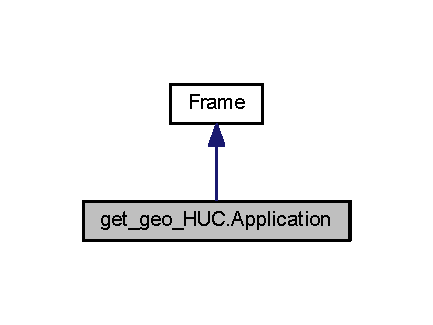
\includegraphics[width=208pt]{classget__geo___h_u_c_1_1_application__inherit__graph}
\end{center}
\end{figure}


Collaboration diagram for get\+\_\+geo\+\_\+\+H\+U\+C.\+Application\+:
\nopagebreak
\begin{figure}[H]
\begin{center}
\leavevmode
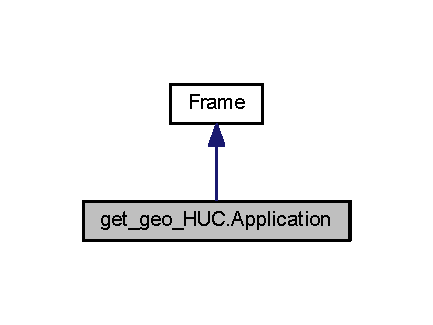
\includegraphics[width=208pt]{classget__geo___h_u_c_1_1_application__coll__graph}
\end{center}
\end{figure}


\subsection{Detailed Description}


Definition at line 14 of file get\+\_\+geo\+\_\+\+H\+U\+C.\+py.



The documentation for this class was generated from the following file\+:\begin{DoxyCompactItemize}
\item 
\hyperlink{get__geo___h_u_c_8py}{get\+\_\+geo\+\_\+\+H\+U\+C.\+py}\end{DoxyCompactItemize}

\hypertarget{class_frame}{}\section{Frame Class Reference}
\label{class_frame}\index{Frame@{Frame}}


Inheritance diagram for Frame\+:
\nopagebreak
\begin{figure}[H]
\begin{center}
\leavevmode
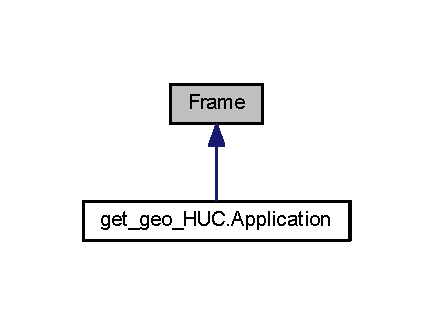
\includegraphics[width=208pt]{class_frame__inherit__graph}
\end{center}
\end{figure}


The documentation for this class was generated from the following file\+:\begin{DoxyCompactItemize}
\item 
\hyperlink{get__geo___h_u_c_8py}{get\+\_\+geo\+\_\+\+H\+U\+C.\+py}\end{DoxyCompactItemize}

\hypertarget{classget__geo___h_u_c_1_1geo}{}\section{get\+\_\+geo\+\_\+\+H\+U\+C.\+geo Class Reference}
\label{classget__geo___h_u_c_1_1geo}\index{get\+\_\+geo\+\_\+\+H\+U\+C.\+geo@{get\+\_\+geo\+\_\+\+H\+U\+C.\+geo}}


\subsection{Detailed Description}


Definition at line 89 of file get\+\_\+geo\+\_\+\+H\+U\+C.\+py.



The documentation for this class was generated from the following file\+:\begin{DoxyCompactItemize}
\item 
\hyperlink{get__geo___h_u_c_8py}{get\+\_\+geo\+\_\+\+H\+U\+C.\+py}\end{DoxyCompactItemize}

\chapter{File Documentation}
\hypertarget{get__geo___h_u_c_8py}{}\section{get\+\_\+geo\+\_\+\+H\+U\+C.\+py File Reference}
\label{get__geo___h_u_c_8py}\index{get\+\_\+geo\+\_\+\+H\+U\+C.\+py@{get\+\_\+geo\+\_\+\+H\+U\+C.\+py}}
\subsection*{Classes}
\begin{DoxyCompactItemize}
\item 
class \hyperlink{classget__geo___h_u_c_1_1_application}{get\+\_\+geo\+\_\+\+H\+U\+C.\+Application}
\item 
class \hyperlink{classget__geo___h_u_c_1_1geo}{get\+\_\+geo\+\_\+\+H\+U\+C.\+geo}
\end{DoxyCompactItemize}
\subsection*{Namespaces}
\begin{DoxyCompactItemize}
\item 
 \hyperlink{namespaceget__geo___h_u_c}{get\+\_\+geo\+\_\+\+H\+UC}
\end{DoxyCompactItemize}
\subsection*{Functions}
\begin{DoxyCompactItemize}
\item 
def \hyperlink{namespaceget__geo___h_u_c_a00508deb9e21d5ff5be209dada8cb9fd}{get\+\_\+geo\+\_\+\+H\+U\+C.\+create\+Widgets} (self)
\item 
def \hyperlink{namespaceget__geo___h_u_c_a400d7645bf5f9b8f5a07cd60f749d1b7}{get\+\_\+geo\+\_\+\+H\+U\+C.\+get\+\_\+geo} (self, args)
\item 
def \hyperlink{namespaceget__geo___h_u_c_a4d0dce07eab2a159ef5d04e0742d5e03}{get\+\_\+geo\+\_\+\+H\+U\+C.\+is\+\_\+number} (self, s)
\item 
def \hyperlink{namespaceget__geo___h_u_c_a4464d7f0ff14cfe91f0b14a490327af9}{get\+\_\+geo\+\_\+\+H\+U\+C.\+\_\+\+\_\+init\+\_\+\+\_\+} (self, master=None)
\item 
def \hyperlink{namespaceget__geo___h_u_c_ab68d25f6902e2500c520513afb9253f2}{get\+\_\+geo\+\_\+\+H\+U\+C.\+geocode} (self, latlng, sensor, geo\+\_\+args)
\item 
def \hyperlink{namespaceget__geo___h_u_c_ad7a7e36924d7182d2e06569e3abb5ea7}{get\+\_\+geo\+\_\+\+H\+U\+C.\+huccode} (self, dms\+\_\+lat, dms\+\_\+lon, huc\+\_\+args)
\item 
def \hyperlink{namespaceget__geo___h_u_c_ace8718ec9f6ab42ef73d183f38576100}{get\+\_\+geo\+\_\+\+H\+U\+C.\+convert\+\_\+dms} (self, d, m, s)
\item 
def \hyperlink{namespaceget__geo___h_u_c_a79b57d5406de0fef5ee616514de74584}{get\+\_\+geo\+\_\+\+H\+U\+C.\+convert\+\_\+dec\+\_\+tude} (self, decimal)
\item 
def \hyperlink{namespaceget__geo___h_u_c_a25d58c7f5b75b8d09a4738ec01a0e312}{get\+\_\+geo\+\_\+\+H\+U\+C.\+convert\+\_\+dec\+\_\+lat\+\_\+lon} (self, decimal, tude)
\end{DoxyCompactItemize}
\subsection*{Variables}
\begin{DoxyCompactItemize}
\item 
\hyperlink{namespaceget__geo___h_u_c_a7592d1dc926835f8c651c5761a3cf94a}{get\+\_\+geo\+\_\+\+H\+U\+C.\+location}
\item 
\hyperlink{namespaceget__geo___h_u_c_ada77bf554a2fd51d028bc3830983b8b6}{get\+\_\+geo\+\_\+\+H\+U\+C.\+text}
\item 
\hyperlink{namespaceget__geo___h_u_c_aa7eddbf5988aec86b6750fa36bf532be}{get\+\_\+geo\+\_\+\+H\+U\+C.\+e}
\item 
\hyperlink{namespaceget__geo___h_u_c_a5d34137420af63fc8dd32374dead14a8}{get\+\_\+geo\+\_\+\+H\+U\+C.\+self}
\item 
\hyperlink{namespaceget__geo___h_u_c_ad4f932dfe1b13e5124bc8be92dfb1f07}{get\+\_\+geo\+\_\+\+H\+U\+C.\+width}
\item 
\hyperlink{namespaceget__geo___h_u_c_a6756d51ec2f6d391eddbc37c88a3369c}{get\+\_\+geo\+\_\+\+H\+U\+C.\+b}
\item 
\hyperlink{namespaceget__geo___h_u_c_a8aad6d9263e79de308254e23bad82c50}{get\+\_\+geo\+\_\+\+H\+U\+C.\+command}
\item 
\hyperlink{namespaceget__geo___h_u_c_a49b3d33e0540c2e2f9e991370aae8f8e}{get\+\_\+geo\+\_\+\+H\+U\+C.\+cnty\+\_\+lab}
\item 
\hyperlink{namespaceget__geo___h_u_c_a3cbe3b2d0670a061bbc0c7be84c34d33}{get\+\_\+geo\+\_\+\+H\+U\+C.\+result} = geo.\+simplejson.\+load(geo.\+urllib.\+urlopen(url))
\item 
\hyperlink{namespaceget__geo___h_u_c_a5e43010bf41ec0eb1eb43403e310e26e}{get\+\_\+geo\+\_\+\+H\+U\+C.\+t}
\item 
\hyperlink{namespaceget__geo___h_u_c_ac67b3377ef85a8077485ef5ae2c64c59}{get\+\_\+geo\+\_\+\+H\+U\+C.\+textvariable}
\item 
\hyperlink{namespaceget__geo___h_u_c_adae93ea1e2d42a6d3c9992ae2e2277a0}{get\+\_\+geo\+\_\+\+H\+U\+C.\+huc\+\_\+lab}
\item 
\hyperlink{namespaceget__geo___h_u_c_a68717ed78e37a7292f01cf4e97c95e9f}{get\+\_\+geo\+\_\+\+H\+U\+C.\+huc\+\_\+var}
\item 
\hyperlink{namespaceget__geo___h_u_c_a0ac336639aa6dc23f2920f162311021b}{get\+\_\+geo\+\_\+\+H\+U\+C.\+t\+\_\+huc}
\item 
\hyperlink{namespaceget__geo___h_u_c_acafcc8295c3d6a0de2fb561809cca132}{get\+\_\+geo\+\_\+\+H\+U\+C.\+latlng} = self.\+contents.\+get().replace(\textquotesingle{} \textquotesingle{}, \textquotesingle{}\textquotesingle{})
\item 
\hyperlink{namespaceget__geo___h_u_c_a299ab467b6f9c8780c7b107ebf7681f3}{get\+\_\+geo\+\_\+\+H\+U\+C.\+dec\+\_\+lat} = float(latlng\mbox{[}\+:latlng.\+find(\textquotesingle{},\textquotesingle{})\mbox{]})
\item 
\hyperlink{namespaceget__geo___h_u_c_afbfb5c7891caec4cd76fe21058d6e7ad}{get\+\_\+geo\+\_\+\+H\+U\+C.\+dec\+\_\+lon} = float(latlng\mbox{[}latlng.\+find(\textquotesingle{},\textquotesingle{})+1\+:\mbox{]})
\item 
\hyperlink{namespaceget__geo___h_u_c_ac22be281ee4954369c420f4045ec3336}{get\+\_\+geo\+\_\+\+H\+U\+C.\+dms\+\_\+lat} = geo.\+convert\+\_\+dec\+\_\+lat\+\_\+lon(g, dec\+\_\+lat, \textquotesingle{}lat\textquotesingle{})
\item 
\hyperlink{namespaceget__geo___h_u_c_a3db416386a0a3ae6cf4b30fab0f65118}{get\+\_\+geo\+\_\+\+H\+U\+C.\+dms\+\_\+lon} = geo.\+convert\+\_\+dec\+\_\+lat\+\_\+lon(g, dec\+\_\+lon, \textquotesingle{}lon\textquotesingle{})
\item 
\hyperlink{namespaceget__geo___h_u_c_a522c7169970f8e82ad010316aad9dfb2}{get\+\_\+geo\+\_\+\+H\+U\+C.\+cnty\+\_\+state} = \textquotesingle{}\textquotesingle{}
\item 
\hyperlink{namespaceget__geo___h_u_c_a1619e8221c4336ab1e3f9c06c3481806}{get\+\_\+geo\+\_\+\+H\+U\+C.\+g} = geo()
\item 
\hyperlink{namespaceget__geo___h_u_c_abd10e556b8081f3cd80bff1a987455af}{get\+\_\+geo\+\_\+\+H\+U\+C.\+sensor}
\item 
\hyperlink{namespaceget__geo___h_u_c_ab14c44a4718f2c2eb40b85e71e76a77a}{get\+\_\+geo\+\_\+\+H\+U\+C.\+huc}
\item 
\hyperlink{namespaceget__geo___h_u_c_a7aa1af4577a3ac49f7c1b8ff5e1c88e8}{get\+\_\+geo\+\_\+\+H\+U\+C.\+G\+E\+O\+C\+O\+D\+E\+\_\+\+B\+A\+S\+E\+\_\+\+U\+RL} = \textbackslash{}
\item 
string \hyperlink{namespaceget__geo___h_u_c_ab6098a8720c14d3cf3f34a3301c2ca93}{get\+\_\+geo\+\_\+\+H\+U\+C.\+url} = G\+E\+O\+C\+O\+D\+E\+\_\+\+B\+A\+S\+E\+\_\+\+U\+RL+\textquotesingle{}?\textquotesingle{}
\item 
\hyperlink{namespaceget__geo___h_u_c_a55007b40146df8c34c3848a9944800d0}{get\+\_\+geo\+\_\+\+H\+U\+C.\+types}
\item 
\hyperlink{namespaceget__geo___h_u_c_abc778873c4005f461907aeb3d7e5c567}{get\+\_\+geo\+\_\+\+H\+U\+C.\+result2} = geo.\+simplejson.\+loads(types)
\item 
string \hyperlink{namespaceget__geo___h_u_c_aec26fed42e6a2aa5dd3adef771e80f56}{get\+\_\+geo\+\_\+\+H\+U\+C.\+H\+U\+C\+\_\+\+B\+A\+S\+E\+\_\+\+U\+RL} = \textquotesingle{}http\+://water.\+usgs.\+gov/cgi-\/bin/pointinhuc.\+pl\textquotesingle{}
\item 
string \hyperlink{namespaceget__geo___h_u_c_a116c62a95390733e5851cce08e203e01}{get\+\_\+geo\+\_\+\+H\+U\+C.\+huc\+\_\+url} = H\+U\+C\+\_\+\+B\+A\+S\+E\+\_\+\+U\+RL+\textquotesingle{}?\textquotesingle{}
\item 
\hyperlink{namespaceget__geo___h_u_c_a9a9f27e6a575181fcea56a1baed08456}{get\+\_\+geo\+\_\+\+H\+U\+C.\+page} = geo.\+urllib.\+urlopen(huc\+\_\+url).read()
\item 
\hyperlink{namespaceget__geo___h_u_c_a7d1d839fc837e44e52f5fba440d56faa}{get\+\_\+geo\+\_\+\+H\+U\+C.\+index} = page.\+find(\textquotesingle{}U\+S\+GS Cataloging Unit\+:\textquotesingle{})
\item 
\hyperlink{namespaceget__geo___h_u_c_a67ca2e90497c71a6704c6755bca3082b}{get\+\_\+geo\+\_\+\+H\+U\+C.\+huc\+\_\+num} = page\mbox{[}index\+:index+35\mbox{]}
\item 
\hyperlink{namespaceget__geo___h_u_c_a0e71504390ae6e1820bf73cf9cbc149f}{get\+\_\+geo\+\_\+\+H\+U\+C.\+num\+\_\+index} = huc\+\_\+num.\+find(\textquotesingle{}\+:\textquotesingle{})
\item 
\hyperlink{namespaceget__geo___h_u_c_abade12bbf1229daaa34a0760a56ef195}{get\+\_\+geo\+\_\+\+H\+U\+C.\+huc\+\_\+name} = page\mbox{[}index\+:index+80\mbox{]}
\item 
int \hyperlink{namespaceget__geo___h_u_c_aa6c84e39c9fc06d8d30722ddc165d320}{get\+\_\+geo\+\_\+\+H\+U\+C.\+dec\+\_\+sec} = s/60
\item 
int \hyperlink{namespaceget__geo___h_u_c_a1cfdb988f3eb1e0c20b5d08ce96d901d}{get\+\_\+geo\+\_\+\+H\+U\+C.\+dec\+\_\+m} = m/60
\item 
\hyperlink{namespaceget__geo___h_u_c_a37be49575af3bb798889e4fcce1f79fe}{get\+\_\+geo\+\_\+\+H\+U\+C.\+dec\+\_\+d} = d+dec\+\_\+m+dec\+\_\+sec
\item 
\hyperlink{namespaceget__geo___h_u_c_adb089a41ce48669080941422b65583fc}{get\+\_\+geo\+\_\+\+H\+U\+C.\+degrees} = int(decimal)
\item 
\hyperlink{namespaceget__geo___h_u_c_a14d62b5f7d112b3f57e1e8dca6ef5dee}{get\+\_\+geo\+\_\+\+H\+U\+C.\+frac} = decimal-\/degrees
\item 
\hyperlink{namespaceget__geo___h_u_c_a8aeb9eaada16136431fe16303cf97135}{get\+\_\+geo\+\_\+\+H\+U\+C.\+minutes} = int(60 $\ast$ frac)
\item 
\hyperlink{namespaceget__geo___h_u_c_a8aacd0fb25a1b4019c52fe5375534130}{get\+\_\+geo\+\_\+\+H\+U\+C.\+m\+\_\+str} = str(minutes)
\item 
\hyperlink{namespaceget__geo___h_u_c_aa2aecbc23891c0a903200e79ea8aed8a}{get\+\_\+geo\+\_\+\+H\+U\+C.\+seconds} = int((frac $\ast$ 3600) \% 60)
\item 
\hyperlink{namespaceget__geo___h_u_c_a48fac2a37a1bbe32015504a0dc9f6c59}{get\+\_\+geo\+\_\+\+H\+U\+C.\+s\+\_\+str} = str(seconds)
\item 
\hyperlink{namespaceget__geo___h_u_c_ab1c89ec30aacba4c19305db584b1da12}{get\+\_\+geo\+\_\+\+H\+U\+C.\+dms} = str(degrees)+m\+\_\+str+s\+\_\+str
\item 
string \hyperlink{namespaceget__geo___h_u_c_a889ac010fb56a383bcd7632fea041a9e}{get\+\_\+geo\+\_\+\+H\+U\+C.\+char} = \textquotesingle{}S\textquotesingle{}
\item 
\hyperlink{namespaceget__geo___h_u_c_a938476c6ba710cee3c941c3def8456a8}{get\+\_\+geo\+\_\+\+H\+U\+C.\+root} = Tk()
\item 
\hyperlink{namespaceget__geo___h_u_c_ae7441cdd21124e2861a4383ed6aa35dd}{get\+\_\+geo\+\_\+\+H\+U\+C.\+app} = Application(master=root)
\item 
\hyperlink{namespaceget__geo___h_u_c_a64b97d57e591931c5f39709ac5d83dad}{get\+\_\+geo\+\_\+\+H\+U\+C.\+contents}
\end{DoxyCompactItemize}

%--- End generated contents ---

% Index
\backmatter
\newpage
\phantomsection
\clearemptydoublepage
\addcontentsline{toc}{chapter}{Index}
\printindex

\end{document}
